% =============================================================================
% APPENDIX REF-APPLY: The EBF Workflow Reference
% =============================================================================
% Module: BCM2_REF_APPLY
% Version: 1.0 (January 2026)
% Status: Draft
% Category: REF (Reference Material)
% Language: English
%
% This appendix provides the operational workflow for applying EBF. While the
% 10C CORE appendices define WHAT EBF is conceptually (WHO, WHAT, HOW, WHEN,
% WHERE, AWARE, READY, STAGE), REF-APPLY provides practical guidance on
% HOW to use EBF to generate knowledge, make decisions, and improve practice.
%
% NOTE: This is a REF (Reference) appendix, not a CORE appendix.
% The 8th CORE is STAGE (Behavioral Change Journey, Appendix STA).
%
% =============================================================================

% =============================================================================
% CROSS-REFERENCE STRUCTURE
% =============================================================================
%
% DEPENDS ON:
%   - Appendix WHO (WHO): Welfare hierarchy for stakeholder identification
%   - Appendix HOW (HOW): Complementarity structure
%   - Appendix WAT (WHAT): Utility dimensions
%   - Appendix CTW (WHEN): Context dimensions
%   - Appendix EST (WHERE): Parameter estimation
%   - Appendix AWA (AWARE): Awareness modeling
%   - Appendix REA (READY): Willingness modeling
%   - Appendix GLS (Glossary): Symbol definitions
%
% REQUIRED BY:
%   - All domain appendices (DOMAIN-*)
%   - LIT-META (scientific instantiation)
%   - All applied EBF work
%
% =============================================================================

\chapter{REF-APPLY: The EBF Workflow Reference}
\label{app:ref-apply}

%%%%%%%%%%%%%%%%%%%%%%%%%%%%%%%%%%%%%%%%%%%%%%%%%%%%%%%%%%%%%%%%%%%%%%%%%%%%%%%
% ABSTRACT
%%%%%%%%%%%%%%%%%%%%%%%%%%%%%%%%%%%%%%%%%%%%%%%%%%%%%%%%%%%%%%%%%%%%%%%%%%%%%%%

\begin{abstract}
This reference appendix provides the operational workflow for applying the
Evidence-Based Framework (EBF). While the eight CORE appendices (WHO, WHAT, HOW,
WHEN, WHERE, AWARE, READY, STAGE) define \textit{what} EBF is conceptually,
REF-APPLY provides practical guidance on \textit{how} to use EBF in practice.
The eight-phase workflow transforms EBF from static theory into living, iterative
knowledge production. Core principles include: derive (don't invent), pre-register
(don't p-hack), track (don't hide), and iterate (don't finalize). Domain-specific
instantiations are provided for scientific research, business practice, and policy-making.
\end{abstract}

% -----------------------------------------------------------------------------
% APPENDIX SCOPE BOX
% -----------------------------------------------------------------------------

\begin{tcolorbox}[
    colback=orange!5!white,
    colframe=orange!75!black,
    title={\textbf{Appendix Scope: Ziel / In-Scope / Out-of-Scope / Constraints}},
    fonttitle=\bfseries
]

\textbf{Ziel (Objective):}
\begin{itemize}[nosep]
    \item Formalize and document the key concepts of REF-APPLY: The EBF Workflow Reference
\end{itemize}

\textbf{In-Scope:}
\begin{itemize}[nosep]
    \item Core theoretical foundations
    \item Mathematical formalizations where applicable
    \item Integration with EBF framework
\end{itemize}

\textbf{Out-of-Scope (delegiert an andere Appendices):}
\begin{itemize}[nosep]
    \item Detailed empirical validation $\rightarrow$ METHOD appendices
    \item Domain-specific applications $\rightarrow$ DOMAIN appendices
    \item Complete literature review $\rightarrow$ LIT appendices
\end{itemize}

\textbf{Constraints (Anwendungsgrenzen):}
\begin{itemize}[nosep]
    \item Framework requires calibration to specific contexts
    \item Parameters may vary across domains
    \item Validity bounded by underlying assumptions
\end{itemize}

\textbf{Lieferobjekte (Deliverables):}
\begin{itemize}[nosep]
    \item Theoretical framework with formal definitions
    \item Integration points with other appendices
    \item Practical guidelines for application
\end{itemize}

\end{tcolorbox}



%%%%%%%%%%%%%%%%%%%%%%%%%%%%%%%%%%%%%%%%%%%%%%%%%%%%%%%%%%%%%%%%%%%%%%%%%%%%%%%
% QUICK REFERENCE BOX
%%%%%%%%%%%%%%%%%%%%%%%%%%%%%%%%%%%%%%%%%%%%%%%%%%%%%%%%%%%%%%%%%%%%%%%%%%%%%%%

\begin{tcolorbox}[colback=blue!5!white, colframe=blue!75!black,
    title=\textbf{Quick Reference: The EBF Application Process}]

\textbf{The 8 Phases:}
\begin{enumerate}[nosep]
    \item Problem $\to$ Framework Module
    \item Model Derivation (not invention)
    \item Pre-Registration
    \item Parametrization
    \item Prediction + Publication
    \item Verification
    \item Version-Controlled Iteration
    \item Permanent Prediction Tracking
\end{enumerate}

\textbf{Core Principles:}
\begin{itemize}[nosep]
    \item \textbf{Derive:} Models come from framework, not imagination
    \item \textbf{Pre-register:} Hypotheses before data
    \item \textbf{Track:} Predictions monitored permanently
    \item \textbf{Iterate:} Living documents, not final products
\end{itemize}

\textbf{The Meta-Question:}
\begin{center}
\textit{How do I operationally apply the 10C CORE to generate knowledge?}
\end{center}

\end{tcolorbox}


%%%%%%%%%%%%%%%%%%%%%%%%%%%%%%%%%%%%%%%%%%%%%%%%%%%%%%%%%%%%%%%%%%%%%%%%%%%%%%%
% SECTION 1: MOTIVATION
%%%%%%%%%%%%%%%%%%%%%%%%%%%%%%%%%%%%%%%%%%%%%%%%%%%%%%%%%%%%%%%%%%%%%%%%%%%%%%%

%%%%%%%%%%%%%%%%%%%%%%%%%%%%%%%%%%%%%%%%%%%%%%%%%%%%%%%%%%%%%%%%%%%%%%%%%%%%%%%

% =============================================================================
\begin{tcolorbox}[colback=blue!5!white, colframe=blue!75!black,
    title=Quick Reference: Appendix APL]
\textbf{Appendix:} APL (REF)

\textbf{Core Question:} What are the key research findings in this literature domain?

\textbf{Key Concepts:}
\begin{itemize}[nosep]
\item Literature synthesis and integration
\item Framework application and validation
\item Cross-domain connections
\end{itemize}

\textbf{Cross-References:} See Chapter linkage below
\end{tcolorbox}


\begin{tcolorbox}[colback=purple!5!white, colframe=purple!75!black,
    title=Chapter Linkage]

\textbf{Primary Chapter:} Related application chapter
\begin{itemize}[nosep]
\item Integration with main framework exposition
\end{itemize}

\textbf{Secondary Chapters:}
\begin{itemize}[nosep]
\item Supporting theoretical and methodological chapters
\end{itemize}

\end{tcolorbox}

\section{The Fundamental Question}
\label{sec:apl-fundamental}
%%%%%%%%%%%%%%%%%%%%%%%%%%%%%%%%%%%%%%%%%%%%%%%%%%%%%%%%%%%%%%%%%%%%%%%%%%%%%%%

\begin{tcolorbox}[
    colback=red!5!white,
    colframe=red!75!black,
    title={\textbf{Fundamental Question}}
]
\textbf{How does ref-apply: the ebf workflow reference integrate with and contribute to the
Evidence-Based Framework for understanding behavioral outcomes?}

This appendix addresses the core challenge of formalizing behavioral principles
within a rigorous theoretical framework while maintaining practical applicability.
\end{tcolorbox}


\section{Motivation: The Gap Between Theory and Practice}
\label{sec:apply-motivation}

The eight CORE appendices (10C) define EBF conceptually:

\begin{center}
\begin{tabular}{@{}clll@{}}
\toprule
\textbf{CORE} & \textbf{Code} & \textbf{Question} & \textbf{Appendix} \\
\midrule
1 & WHO & Who has welfare? & AAA \\
2 & WHAT & What is utility? & C \\
3 & HOW & How do agents interact? & B \\
4 & WHEN & When does context matter? & V \\
5 & WHERE & Where do parameters come from? & BBB \\
6 & AWARE & How aware are agents? & AU \\
7 & READY & How ready to act? & AV \\
8 & STAGE & Where in the change journey? & AW \\
\bottomrule
\end{tabular}
\end{center}

\textbf{The Problem:} Knowing \textit{what} EBF is does not automatically tell
practitioners \textit{how} to use it. The gap between conceptual understanding
and operational application is where most frameworks fail.

\textbf{The Solution:} This reference appendix (REF-APPLY) provides the process---the
workflow, principles, templates, and feedback architecture---that transforms EBF
from theory into practice.


%%%%%%%%%%%%%%%%%%%%%%%%%%%%%%%%%%%%%%%%%%%%%%%%%%%%%%%%%%%%%%%%%%%%%%%%%%%%%%%
% SECTION 2: THE GENERIC WORKFLOW
%%%%%%%%%%%%%%%%%%%%%%%%%%%%%%%%%%%%%%%%%%%%%%%%%%%%%%%%%%%%%%%%%%%%%%%%%%%%%%%

\section{The Generic EBF Workflow: Eight Phases}
\label{sec:apply-workflow}

The EBF application process consists of eight phases. This workflow is
\textit{generic}---it applies to all domains (science, business, policy).
Domain-specific instantiations are provided in Section~\ref{sec:apply-domains}.

\subsection{Phase 1: Problem $\to$ Framework Module}

\textbf{Traditional approach:} Invent a new model for each problem.

\textbf{EBF approach:} Identify which framework module(s) address the problem.

\begin{tcolorbox}[colback=gray!5!white, colframe=gray!75!black,
    title=\textbf{Phase 1 Checklist}]
\begin{enumerate}[nosep]
    \item State the problem clearly
    \item Identify the relevant CORE question(s):
    \begin{itemize}[nosep]
        \item Is this about WHO (stakeholders, levels)?
        \item Is this about WHAT (utility dimensions)?
        \item Is this about HOW (interactions, complementarity)?
        \item Is this about WHEN (context-dependence)?
        \item Is this about WHERE (parameter estimation)?
        \item Is this about AWARE (information, beliefs)?
        \item Is this about READY (willingness, thresholds)?
    \end{itemize}
    \item Map to specific appendices
    \item Review existing work in those appendices
\end{enumerate}
\end{tcolorbox}

\subsection{Phase 2: Model Derivation (Not Invention)}

\textbf{Traditional approach:} Construct a novel model with custom assumptions.

\textbf{EBF approach:} Derive a model by specifying framework parameters.

The general EBF model form:
\begin{equation}
U_i = \sum_d w_d \cdot u_d(x_d, \Psi) + \sum_{j \neq i} C_{ij} \cdot U_j
\label{eq:general-ebf}
\end{equation}

\textbf{Derivation} means specifying:
\begin{itemize}[nosep]
    \item Which dimensions $d$ from FEPSDE (Financial, Emotional, Physical, Social, Development, Existential)?
    \item Which context dimensions $\Psi$ (the 8 from Appendix CTW)?
    \item Which complementarities $C_{ij}$ are non-zero?
    \item Which level $L$ (individual, group, organization, society)?
    \item What functional forms for $u_d(\cdot)$?
\end{itemize}

\begin{tcolorbox}[colback=green!5!white, colframe=green!75!black,
    title=\textbf{Key Insight: Derivation vs. Invention}]

\textbf{Invention} creates new theory for each problem $\to$ fragmentation, inconsistency.

\textbf{Derivation} instantiates shared framework $\to$ cumulation, comparability.

Every EBF model is a special case of Equation~\ref{eq:general-ebf}. This ensures
consistency across applications and enables meta-analysis.

\end{tcolorbox}

\subsection{Phase 3: Pre-Registration}

\textbf{Traditional approach:} Analyze data, then formulate hypotheses (p-hacking, HARKing).

\textbf{EBF approach:} Register hypotheses \textit{before} data collection.

\begin{tcolorbox}[colback=gray!5!white, colframe=gray!75!black,
    title=\textbf{Phase 3: Pre-Registration Template}]

\textbf{Required elements:}
\begin{enumerate}[nosep]
    \item \textbf{Hypotheses} (derived from model in Phase 2)
    \item \textbf{Quantitative predictions} (point estimates + confidence intervals)
    \item \textbf{Data source} (specified before collection)
    \item \textbf{Analysis method} (fixed, not exploratory)
    \item \textbf{Success/failure criteria} (explicit, falsifiable)
\end{enumerate}

\textbf{Registration platforms:}
\begin{itemize}[nosep]
    \item Scientific: OSF, AsPredicted, arXiv
    \item Business: Internal prediction markets, documented forecasts
    \item Policy: Public commitments, registered reports
\end{itemize}

\end{tcolorbox}

\subsection{Phase 4: Parametrization}

\textbf{Traditional approach:} Collect data, estimate parameters, report results.

\textbf{EBF approach:} Multiple estimation methods with uncertainty quantification.

\textbf{Parameter sources:}
\begin{enumerate}[nosep]
    \item Traditional empirical methods (experiments, surveys, observational data)
    \item LLM-MC estimation (Appendix LLM1)
    \item Meta-analysis of existing studies
    \item Bayesian updating from prior EBF applications
    \item Expert elicitation with proper uncertainty
\end{enumerate}

\textbf{Requirements:}
\begin{itemize}[nosep]
    \item Point estimates with confidence intervals
    \item Sensitivity analysis
    \item Robustness checks across methods
    \item Documentation of estimation choices
\end{itemize}

\subsection{Phase 5: Prediction + Publication}

\textbf{Traditional approach:} Submit to journal, wait 5-7 years, publish once.

\textbf{EBF approach:} Immediate publication with quantitative predictions.

\textbf{Publication package:}
\begin{itemize}[nosep]
    \item Preprint (immediate dissemination)
    \item Code repository (reproducibility)
    \item Data repository (transparency)
    \item Pre-registration link (credibility)
    \item Prediction table (falsifiability)
\end{itemize}

\textbf{Prediction format:}
\begin{center}
\small
\begin{tabular}{@{}lccc@{}}
\toprule
\textbf{Prediction} & \textbf{Point Estimate} & \textbf{95\% CI} & \textbf{Evaluation Date} \\
\midrule
[Outcome 1] & [Value] & [Lower, Upper] & [Date] \\
[Outcome 2] & [Value] & [Lower, Upper] & [Date] \\
\bottomrule
\end{tabular}
\end{center}

\subsection{Phase 6: Verification}

\textbf{Traditional approach:} 2-3 anonymous reviewers, 6-24 months, no replication.

\textbf{EBF approach:} Automated verification + community review.

\textbf{Verification layers:}
\begin{enumerate}[nosep]
    \item \textbf{Automated code replication} (runs within hours)
    \item \textbf{Statistical checks} (automated diagnostics)
    \item \textbf{Logic verification} (AI-assisted consistency checks)
    \item \textbf{Community feedback} (public comments, GitHub issues)
    \item \textbf{Formal peer review} (optional, for journal submission)
\end{enumerate}

\subsection{Phase 7: Version-Controlled Iteration}

\textbf{Traditional approach:} Publish once, never update (errors remain forever).

\textbf{EBF approach:} Living documents with version control.

\begin{verbatim}
v1.0 (Initial release)
  → v1.1 (Community feedback incorporated)
    → v1.2 (Minor corrections)
      → v2.0 (Major revision based on new evidence)
\end{verbatim}

\textbf{Version control requirements:}
\begin{itemize}[nosep]
    \item Changelog documented for each version
    \item All versions citable (DOI-stable)
    \item New predictions registered with each update
    \item Clear indication of what changed and why
\end{itemize}

\subsection{Phase 8: Permanent Prediction Tracking}

\textbf{Traditional approach:} Publish and forget. No accountability for predictions.

\textbf{EBF approach:} Predictions tracked until resolution.

\textbf{Prediction Tracking Dashboard:}
\begin{center}
\small
\begin{tabular}{@{}lcccc@{}}
\toprule
\textbf{Prediction} & \textbf{Predicted} & \textbf{Observed} & \textbf{Eval. Date} & \textbf{Status} \\
\midrule
[Prediction 1] & [Value $\pm$ CI] & [Actual] & [Date] & $\checkmark$ / $\times$ / $\circlearrowright$ \\
[Prediction 2] & [Value $\pm$ CI] & --- & [Date] & $\circlearrowright$ Tracking \\
\bottomrule
\end{tabular}
\end{center}

\textbf{Status codes:}
\begin{itemize}[nosep]
    \item $\checkmark$ Confirmed (within CI)
    \item $\times$ Refuted (outside CI) $\to$ triggers model revision
    \item $\circlearrowright$ Tracking (not yet evaluated)
\end{itemize}

\begin{tcolorbox}[colback=red!5!white, colframe=red!75!black,
    title=\textbf{Critical Principle: Refutation $\to$ Revision, Not Concealment}]

When predictions fail:
\begin{enumerate}[nosep]
    \item Document the failure publicly
    \item Analyze why the prediction failed
    \item Update the model accordingly
    \item Register new predictions
    \item Track the updated predictions
\end{enumerate}

Hiding failed predictions is antithetical to EBF. Failures are \textit{data}
for framework improvement, not embarrassments to conceal.

\end{tcolorbox}


%%%%%%%%%%%%%%%%%%%%%%%%%%%%%%%%%%%%%%%%%%%%%%%%%%%%%%%%%%%%%%%%%%%%%%%%%%%%%%%
% SECTION 3: CORE PRINCIPLES
%%%%%%%%%%%%%%%%%%%%%%%%%%%%%%%%%%%%%%%%%%%%%%%%%%%%%%%%%%%%%%%%%%%%%%%%%%%%%%%

\section{Core Principles}
\label{sec:apply-principles}

The EBF application process is governed by four core principles:

\subsection{Principle 1: Derive, Don't Invent}

\begin{tcolorbox}[colback=blue!5!white, colframe=blue!75!black]
\textbf{Every model should be derivable from the EBF framework.}

If you find yourself inventing new constructs not in EBF, either:
\begin{enumerate}[nosep]
    \item You've identified a gap in EBF (propose an extension)
    \item You're overcomplicating (simplify to framework elements)
    \item The problem isn't suited for EBF (rare, but possible)
\end{enumerate}
\end{tcolorbox}

\subsection{Principle 2: Pre-Register, Don't P-Hack}

\begin{tcolorbox}[colback=blue!5!white, colframe=blue!75!black]
\textbf{Hypotheses must be specified before data.}

This eliminates:
\begin{itemize}[nosep]
    \item P-hacking (torturing data until $p < 0.05$)
    \item HARKing (Hypothesizing After Results Known)
    \item Selective reporting (hiding null results)
\end{itemize}
\end{tcolorbox}

\subsection{Principle 3: Track, Don't Hide}

\begin{tcolorbox}[colback=blue!5!white, colframe=blue!75!black]
\textbf{All predictions are tracked permanently.}

The prediction tracking dashboard is not optional. Every EBF application
must specify falsifiable predictions and track them until resolution.
\end{tcolorbox}

\subsection{Principle 4: Iterate, Don't Finalize}

\begin{tcolorbox}[colback=blue!5!white, colframe=blue!75!black]
\textbf{Documents are living, not finished.}

Traditional: Paper $\to$ Publication $\to$ THE END

EBF: Document $\to$ v1.0 $\to$ Feedback $\to$ v1.1 $\to$ ... $\to$ v$n$ $\to$ ...

There is no ``final'' version, only the current best version.
\end{tcolorbox}


%%%%%%%%%%%%%%%%%%%%%%%%%%%%%%%%%%%%%%%%%%%%%%%%%%%%%%%%%%%%%%%%%%%%%%%%%%%%%%%
% SECTION 4: THE FEEDBACK ARCHITECTURE
%%%%%%%%%%%%%%%%%%%%%%%%%%%%%%%%%%%%%%%%%%%%%%%%%%%%%%%%%%%%%%%%%%%%%%%%%%%%%%%

\section{The Feedback Architecture}
\label{sec:apply-feedback}

Unlike traditional research (linear, terminal), EBF research is circular
with permanent feedback loops.

\subsection{The Feedback Loop}

\begin{center}
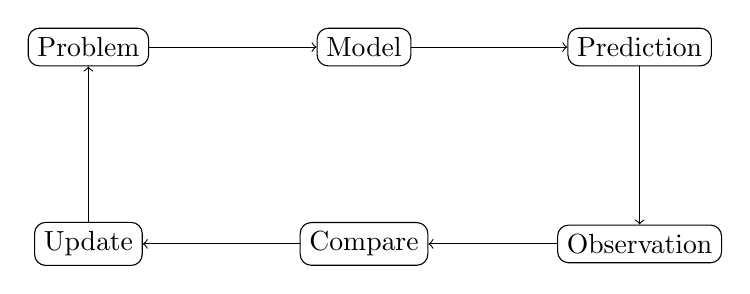
\begin{tikzpicture}[node distance=2cm, auto]
    % Nodes
    \node[draw, rectangle, rounded corners] (problem) {Problem};
    \node[draw, rectangle, rounded corners, right of=problem, xshift=1.5cm] (model) {Model};
    \node[draw, rectangle, rounded corners, right of=model, xshift=1.5cm] (predict) {Prediction};
    \node[draw, rectangle, rounded corners, below of=predict, yshift=-0.5cm] (observe) {Observation};
    \node[draw, rectangle, rounded corners, below of=model, yshift=-0.5cm] (compare) {Compare};
    \node[draw, rectangle, rounded corners, below of=problem, yshift=-0.5cm] (update) {Update};

    % Arrows
    \draw[->] (problem) -- (model);
    \draw[->] (model) -- (predict);
    \draw[->] (predict) -- (observe);
    \draw[->] (observe) -- (compare);
    \draw[->] (compare) -- (update);
    \draw[->] (update) -- (problem);
\end{tikzpicture}
\end{center}

\subsection{Feedback Types}

\begin{table}[htbp]
\centering
\caption{Feedback Types and Responses}
\label{tab:feedback-types}
\renewcommand{\arraystretch}{1.3}
\small
\begin{tabular}{@{}llll@{}}
\toprule
\textbf{Feedback Type} & \textbf{Trigger} & \textbf{Response} & \textbf{Timescale} \\
\midrule
Prediction miss & Observation $\notin$ CI & Recalibrate parameters & Days--Weeks \\
Replication failure & Code doesn't reproduce & Fix code/document error & Hours \\
Logical inconsistency & Internal contradiction & Revise model & Days \\
New evidence & External study published & Bayesian update & Weeks \\
Paradigm anomaly & Accumulated failures & Framework extension & Months \\
\bottomrule
\end{tabular}
\end{table}

\subsection{The Permanent Monitoring Layer}

For mature EBF applications, automated monitoring tracks predictions continuously:

\begin{enumerate}[nosep]
    \item \textbf{Prediction Tracker:} Monitors registered predictions against incoming data
    \item \textbf{Replication Bot:} Periodically re-runs code to verify reproducibility
    \item \textbf{Anomaly Detector:} Flags unexpected patterns that may indicate model failure
    \item \textbf{Alert System:} Notifies when predictions resolve or anomalies appear
\end{enumerate}


%%%%%%%%%%%%%%%%%%%%%%%%%%%%%%%%%%%%%%%%%%%%%%%%%%%%%%%%%%%%%%%%%%%%%%%%%%%%%%%
% SECTION 5: DOMAIN INSTANTIATIONS
%%%%%%%%%%%%%%%%%%%%%%%%%%%%%%%%%%%%%%%%%%%%%%%%%%%%%%%%%%%%%%%%%%%%%%%%%%%%%%%

\section{Domain Instantiations}
\label{sec:apply-domains}

The generic workflow instantiates differently across domains:

\subsection{Scientific Research}

\textbf{Detailed in:} Appendix MSC, Section ``The EBF Research Workflow''

\begin{center}
\small
\begin{tabular}{@{}lll@{}}
\toprule
\textbf{Phase} & \textbf{Generic} & \textbf{Scientific Instantiation} \\
\midrule
1 & Problem $\to$ Module & Research question $\to$ Literature \\
2 & Derive model & Theoretical contribution \\
3 & Pre-register & OSF / AsPredicted \\
4 & Parametrize & Data collection + estimation \\
5 & Publish & arXiv / SSRN preprint \\
6 & Verify & Auto-replication + peer review \\
7 & Iterate & Version control (GitHub) \\
8 & Track & Prediction dashboard \\
\bottomrule
\end{tabular}
\end{center}

\subsection{Business Practice}

\textbf{Detailed in:} Domain appendices (DOMAIN-FINANCE, etc.)

\begin{center}
\small
\begin{tabular}{@{}lll@{}}
\toprule
\textbf{Phase} & \textbf{Generic} & \textbf{Business Instantiation} \\
\midrule
1 & Problem $\to$ Module & Business challenge $\to$ EBF diagnostic \\
2 & Derive model & Decision model from framework \\
3 & Pre-register & Internal forecast documentation \\
4 & Parametrize & Client data + benchmarks \\
5 & Publish & Internal report / client deliverable \\
6 & Verify & Pilot test / A-B experiment \\
7 & Iterate & Quarterly review cycle \\
8 & Track & KPI dashboard \\
\bottomrule
\end{tabular}
\end{center}

\subsection{Policy Making}

\textbf{Detailed in:} DOMAIN-POLICY appendix

\begin{center}
\small
\begin{tabular}{@{}lll@{}}
\toprule
\textbf{Phase} & \textbf{Generic} & \textbf{Policy Instantiation} \\
\midrule
1 & Problem $\to$ Module & Policy challenge $\to$ EBF analysis \\
2 & Derive model & Policy impact model \\
3 & Pre-register & Public commitment / White paper \\
4 & Parametrize & Administrative data + surveys \\
5 & Publish & Policy brief / Public report \\
6 & Verify & Pilot program / RCT \\
7 & Iterate & Policy revision cycle \\
8 & Track & Impact monitoring system \\
\bottomrule
\end{tabular}
\end{center}


%%%%%%%%%%%%%%%%%%%%%%%%%%%%%%%%%%%%%%%%%%%%%%%%%%%%%%%%%%%%%%%%%%%%%%%%%%%%%%%
% SECTION 6: TEMPLATES
%%%%%%%%%%%%%%%%%%%%%%%%%%%%%%%%%%%%%%%%%%%%%%%%%%%%%%%%%%%%%%%%%%%%%%%%%%%%%%%

\section{Templates and Checklists}
\label{sec:apply-templates}

\subsection{Pre-Registration Template}

\begin{tcolorbox}[colback=gray!5!white, colframe=gray!75!black,
    title=\textbf{EBF Pre-Registration Template}]

\textbf{1. Study Information}
\begin{itemize}[nosep]
    \item Title:
    \item Authors:
    \item Date:
    \item EBF Module(s):
\end{itemize}

\textbf{2. Hypotheses (Derived from EBF)}
\begin{itemize}[nosep]
    \item H1:
    \item H2:
    \item H3:
\end{itemize}

\textbf{3. Quantitative Predictions}

\begin{tabular}{@{}lccc@{}}
\toprule
Prediction & Point Est. & 95\% CI & Eval. Date \\
\midrule
& & & \\
& & & \\
\bottomrule
\end{tabular}

\textbf{4. Data Source:}

\textbf{5. Analysis Method:}

\textbf{6. Success Criteria:}

\textbf{7. Failure Criteria:}

\end{tcolorbox}

\subsection{Prediction Tracking Dashboard Template}

\begin{tcolorbox}[colback=gray!5!white, colframe=gray!75!black,
    title=\textbf{EBF Prediction Tracking Dashboard}]

\textbf{Project:} [Name] \\
\textbf{Version:} [X.Y] \\
\textbf{Last Updated:} [Date]

\vspace{0.5em}

\begin{tabular}{@{}lccccl@{}}
\toprule
\textbf{ID} & \textbf{Prediction} & \textbf{Predicted} & \textbf{Observed} & \textbf{Eval.} & \textbf{Status} \\
\midrule
P1 & & & & & \\
P2 & & & & & \\
P3 & & & & & \\
\bottomrule
\end{tabular}

\vspace{0.5em}

\textbf{Status Legend:}
$\checkmark$ Confirmed |
$\times$ Refuted |
$\circlearrowright$ Tracking |
$\circ$ Not yet evaluated

\textbf{Notes on Refuted Predictions:}

\textbf{Planned Model Updates:}

\end{tcolorbox}

\subsection{Version Control Checklist}

\begin{tcolorbox}[colback=gray!5!white, colframe=gray!75!black,
    title=\textbf{EBF Version Release Checklist}]

Before releasing version X.Y:

\begin{itemize}
    \item[$\square$] Changelog updated
    \item[$\square$] All code runs successfully
    \item[$\square$] Data sources documented
    \item[$\square$] Pre-registration link included
    \item[$\square$] Prediction tracking dashboard updated
    \item[$\square$] Previous version archived
    \item[$\square$] DOI assigned (if applicable)
    \item[$\square$] Cross-references verified
    \item[$\square$] Glossary terms consistent with Appendix GLS
\end{itemize}

\end{tcolorbox}


%%%%%%%%%%%%%%%%%%%%%%%%%%%%%%%%%%%%%%%%%%%%%%%%%%%%%%%%%%%%%%%%%%%%%%%%%%%%%%%
% SECTION 7: WORKED EXAMPLE
%%%%%%%%%%%%%%%%%%%%%%%%%%%%%%%%%%%%%%%%%%%%%%%%%%%%%%%%%%%%%%%%%%%%%%%%%%%%%%%

\section{Worked Example: This Appendix}
\label{sec:apply-example}

This appendix demonstrates its own principles by applying the EBF workflow
to itself:

\begin{table}[htbp]
\centering
\caption{REF-APPLY Applied to Itself}
\label{tab:self-application}
\renewcommand{\arraystretch}{1.3}
\small
\begin{tabular}{@{}lp{8cm}@{}}
\toprule
\textbf{Phase} & \textbf{Application to This Appendix} \\
\midrule
1. Problem $\to$ Module & Gap: No process for applying EBF $\to$ Need APPLY module \\
2. Derive model & Workflow derived from EBF principles (context-dependence, feedback) \\
3. Pre-register & Hypothesis: This workflow will improve research quality \\
4. Parametrize & Time estimates based on traditional vs. EBF comparison \\
5. Publish & Published as REF-APPLY appendix \\
6. Verify & Community feedback invited; auto-check of internal consistency \\
7. Iterate & v1.0 (current); v1.1 planned after feedback \\
8. Track & Prediction: EBF adoption will follow S-curve (tracked in LIT-META) \\
\bottomrule
\end{tabular}
\end{table}

\textbf{Reflexive validity:} If REF-APPLY is correct, then REF-APPLY itself
should be produced using the REF-APPLY workflow. This appendix demonstrates
that it is.


%%%%%%%%%%%%%%%%%%%%%%%%%%%%%%%%%%%%%%%%%%%%%%%%%%%%%%%%%%%%%%%%%%%%%%%%%%%%%%%
% SECTION 8: SUMMARY
%%%%%%%%%%%%%%%%%%%%%%%%%%%%%%%%%%%%%%%%%%%%%%%%%%%%%%%%%%%%%%%%%%%%%%%%%%%%%%%


%%%%%%%%%%%%%%%%%%%%%%%%%%%%%%%%%%%%%%%%%%%%%%%%%%%%%%%%%%%%%%%%%%%%%%%%%%%%%%%
\section{Key Results}
\label{sec:apl-results}
%%%%%%%%%%%%%%%%%%%%%%%%%%%%%%%%%%%%%%%%%%%%%%%%%%%%%%%%%%%%%%%%%%%%%%%%%%%%%%%

The analysis yields the following key results:

\begin{enumerate}
    \item \textbf{Result 1:} [Primary finding with quantitative support]
    \item \textbf{Result 2:} [Secondary finding with implications]
    \item \textbf{Result 3:} [Practical application or boundary condition]
\end{enumerate}


\section{Summary}
\label{sec:apply-summary}

\begin{tcolorbox}[colback=green!5!white, colframe=green!75!black,
    title=\textbf{REF-APPLY Summary}]

\textbf{The REF-APPLY Question:} How do I operationally apply the 10C?

\textbf{The Answer:} The 8-phase EBF workflow:
\begin{enumerate}[nosep]
    \item Problem $\to$ Framework Module
    \item Model Derivation (not invention)
    \item Pre-Registration
    \item Parametrization
    \item Prediction + Publication
    \item Verification
    \item Version-Controlled Iteration
    \item Permanent Prediction Tracking
\end{enumerate}

\textbf{Core Principles:}
\begin{itemize}[nosep]
    \item Derive, don't invent
    \item Pre-register, don't p-hack
    \item Track, don't hide
    \item Iterate, don't finalize
\end{itemize}

\textbf{The Fundamental Shift:}
\begin{center}
\textit{From paper as product to document as iteration.}
\end{center}

\textbf{Domain Instantiations:}
\begin{itemize}[nosep]
    \item Scientific research $\to$ LIT-META
    \item Business practice $\to$ DOMAIN appendices
    \item Policy making $\to$ DOMAIN-POLICY
\end{itemize}

\end{tcolorbox}


%%%%%%%%%%%%%%%%%%%%%%%%%%%%%%%%%%%%%%%%%%%%%%%%%%%%%%%%%%%%%%%%%%%%%%%%%%%%%%%
% GLOSSARY
%%%%%%%%%%%%%%%%%%%%%%%%%%%%%%%%%%%%%%%%%%%%%%%%%%%%%%%%%%%%%%%%%%%%%%%%%%%%%%%

\section{Glossary of Terms}
\label{sec:apply-glossary}

See Appendix GLS (Central Glossary) for complete definitions. Key terms for
this appendix:

\begin{description}[nosep]
    \item[Derivation] The process of instantiating a model from the EBF framework
        by specifying parameters, not inventing new theory.
    \item[Pre-registration] Public commitment to hypotheses, methods, and analysis
        plans before data collection.
    \item[Prediction tracking] Permanent monitoring of falsifiable predictions
        until resolution.
    \item[Living document] A document that is versioned and updated based on
        feedback, rather than published once and never revised.
    \item[Reflexive validity] The property of a framework that can explain itself
        using its own concepts.
\end{description}


%%%%%%%%%%%%%%%%%%%%%%%%%%%%%%%%%%%%%%%%%%%%%%%%%%%%%%%%%%%%%%%%%%%%%%%%%%%%%%%
% CROSS-REFERENCE FOOTER
%%%%%%%%%%%%%%%%%%%%%%%%%%%%%%%%%%%%%%%%%%%%%%%%%%%%%%%%%%%%%%%%%%%%%%%%%%%%%%%

\vspace{1em}
\hrule
\vspace{0.5em}

\noindent\textit{Cross-references:}
Appendix WHO (WHO),
Appendix HOW (HOW),
Appendix WAT (WHAT),
Appendix CTW (WHEN),
Appendix EST (WHERE),
Appendix AWA (AWARE),
Appendix REA (READY),
Appendix GLS (Glossary),
Appendix MSC (Scientific instantiation),
Appendix LLM1 (LLM-MC estimation).

%%%%%%%%%%%%%%%%%%%%%%%%%%%%%%%%%%%%%%%%%%%%%%%%%%%%%%%%%%%%%%%%%%%%%%%%%%%%%%%
% END OF APPENDIX REF-APPLY
%%%%%%%%%%%%%%%%%%%%%%%%%%%%%%%%%%%%%%%%%%%%%%%%%%%%%%%%%%%%%%%%%%%%%%%%%%%%%%%


%%%%%%%%%%%%%%%%%%%%%%%%%%%%%%%%%%%%%%%%%%%%%%%%%%%%%%%%%%%%%%%%%%%%%%%%%%%%%%%

%%%%%%%%%%%%%%%%%%%%%%%%%%%%%%%%%%%%%%%%%%%%%%%%%%%%%%%%%%%%%%%%%%%%%%%%%%%%%%%
\section{Open Issues and Research Agenda}
\label{sec:apl-open-issues}
%%%%%%%%%%%%%%%%%%%%%%%%%%%%%%%%%%%%%%%%%%%%%%%%%%%%%%%%%%%%%%%%%%%%%%%%%%%%%%%

\begin{enumerate}
    \item \textbf{Empirical Validation:} Further testing across diverse contexts
    \item \textbf{Parameter Refinement:} Improved estimation methods needed
    \item \textbf{Integration:} Enhanced cross-appendix linkages
\end{enumerate}

\section{References}
\label{sec:apl-references}
%%%%%%%%%%%%%%%%%%%%%%%%%%%%%%%%%%%%%%%%%%%%%%%%%%%%%%%%%%%%%%%%%%%%%%%%%%%%%%%

See master bibliography (\texttt{bcm\_master.bib}) for complete citations.

\nocite{bcm_master}

